\section{Related Works}

\subsection{Introduction to Related Works in DBaaS Systems}
Database-as-a-Service (DBaaS) has emerged as a transformative paradigm in cloud computing, enabling organizations to manage, store, and access data without the need for on-premises infrastructure or dedicated database administrators. In this section, we explore related works in the realm of DBaaS, examining key research, innovative implementations, and industry best practices that have shaped this service model. By reviewing existing literature and case studies, we aim to understand the evolution of DBaaS systems, the architectures employed by major providers, and the practical challenges faced in deploying secure, scalable, and high-performance cloud databases.

We will present a comparative overview of several DBaaS solutions, highlighting their key features, service models, and performance characteristics. This analysis sets the foundation for our proposed DBaaS implementation, guiding the design of a solution optimized for small to medium-sized enterprises (SMEs), balancing performance, scalability, and security in today’s dynamic cloud computing landscape.

% -------------------------------------------------------------------
% DBaaS Longtable
% -------------------------------------------------------------------

\renewcommand{\arraystretch}{1.5} % 1.0 = default, 1.5 = 50% taller rows
\begin{table}[h]  % 'h' means place here, can use t, b, p, etc.
    \centering
    \begin{tabularx}{\textwidth}{|X|c|c|X|c|X|}
    \hline
    \textbf{Platform} & \textbf{SQL} & \textbf{NoSQL} & \textbf{Schema Viz.} & \textbf{Lock-in} & \textbf{AI} \\
    \hline
    
    RDS & \cmark & \xmark & Low & High & \xmark \\
    DynamoDB & \xmark & \cmark & Low & High & \xmark \\
    Google SQL & \cmark & \xmark & Low & High & \xmark \\
    Firesbase & \xmark & \cmark & \xmark & High & \xmark \\
    Azure SQL & \cmark & \xmark & Basic & High & \xmark \\
    Atlas & \xmark & \cmark & Limited & Low & \cmark~(Limited) \\
    PlanetScale & \cmark & \xmark & Limited & Medium & \xmark \\
    NeonDB & \cmark & \xmark & Low & Medium & \xmark \\
    IBM Cloud & \cmark & \cmark & \xmark & High & \xmark \\
    Supabase & \cmark & \xmark & ERD & Medium & \cmark~(Limited) \\
    \hline
    \textbf{Proposed DBaaS} & \textbf{\cmark} & \textbf{\cmark} & \textbf{Full Visual Builder} & \textbf{Low} & \textbf{\cmark~(Full)} \\
    \hline
    \end{tabularx}
    \caption{Comparison of different DBaaS platforms across key features}
    \label{tab:dbaas_comparison}
\end{table}


\subsection{Comparison of Cloud Database Services}

\subsubsection{Amazon RDS}
Amazon RDS functions as a managed relational database that sits in the cloud and connects directly to your application servers. The application interacts with RDS using standard SQL queries over a secure connection. Amazon handles the infrastructure underneath, including storage, CPU, memory, backups, and replication. For high availability, RDS can replicate data across multiple availability zones, and read replicas can serve read-heavy workloads. Essentially, your application only sees a database endpoint; the scaling, maintenance, and failover are abstracted away.
\begin{figure}[H]
    \centering
    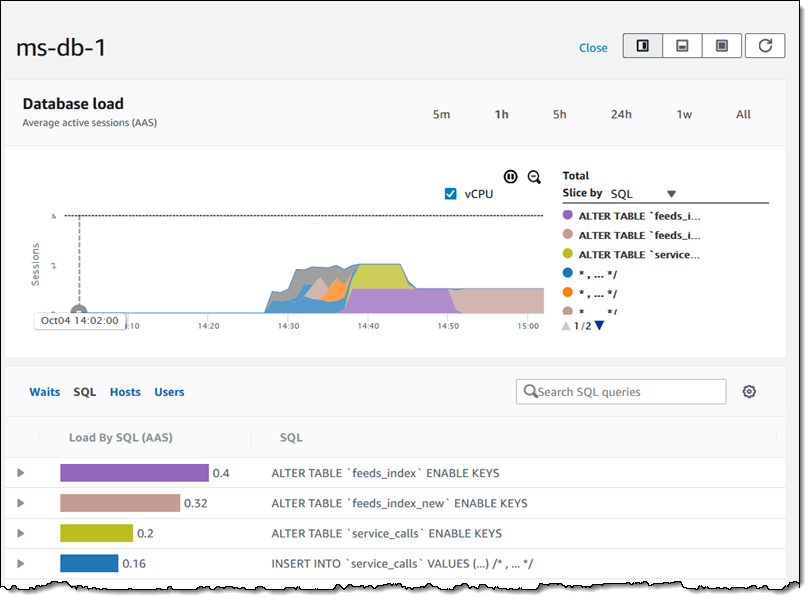
\includegraphics[width=0.85\textwidth]{images/related-work/aws_rds.png}
    \caption{Amazon RDS console} 
    \label{fig:related_aws_rds}
\end{figure}

\subsubsection{Azure SQL Database}
Azure SQL Database works similarly, acting as a fully managed SQL Server in the cloud. Applications connect using T-SQL through standard database drivers or APIs. Azure manages the underlying infrastructure, scaling, patching, and replication. It can operate in serverless mode, where compute scales automatically based on demand, or provisioned mode for predictable workloads. The database is accessible through secure endpoints, and geo-replication allows global applications to read and write data efficiently.
\begin{figure}[H]
    \centering
    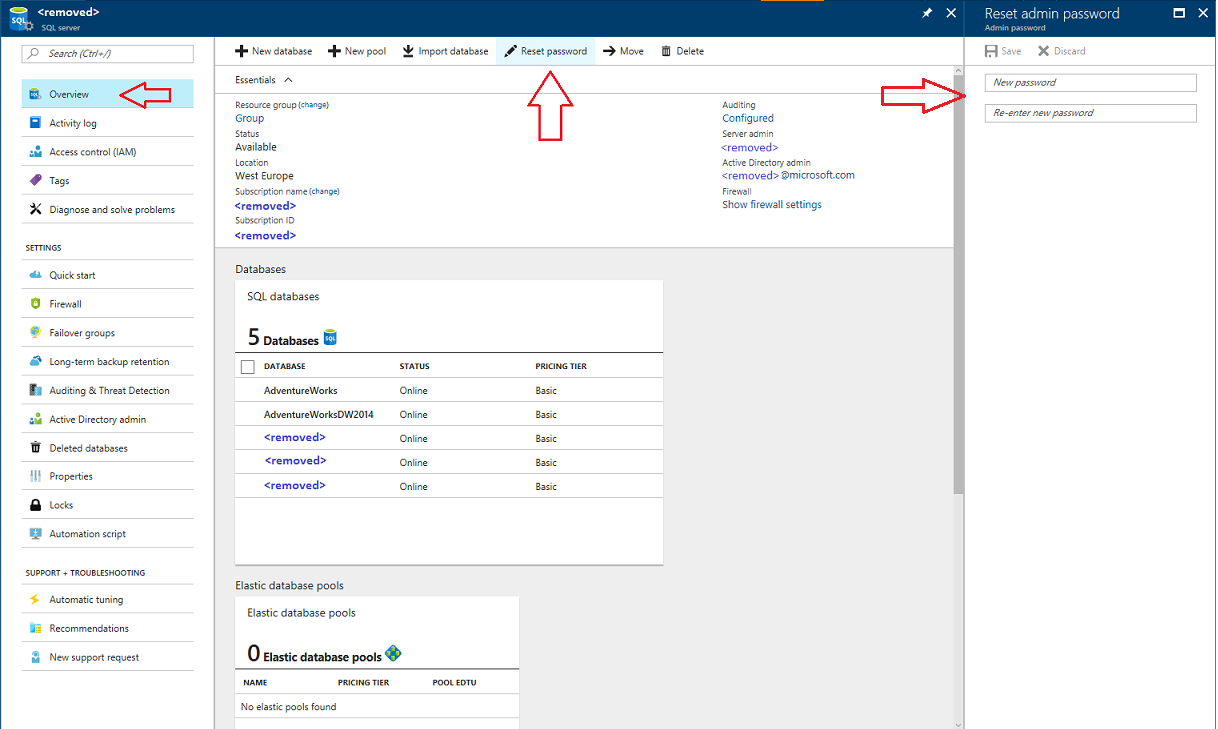
\includegraphics[width=0.85\textwidth]{images/related-work/azure.png}
    \caption{Azure SQL Database console}
    \label{fig:related_azure_sql}
\end{figure}
\subsubsection{MongoDB Atlas}
MongoDB Atlas is a cloud-hosted, document-based NoSQL database. Applications communicate with Atlas using MongoDB drivers or APIs, sending queries in the MongoDB Query Language. Atlas handles sharding and replication in the background, distributing data across multiple nodes or regions to provide scalability and resilience. Because it is schema-less, applications can store and retrieve complex, nested JSON documents without rigid schemas. Global clusters allow users from different regions to access data with low latency.
\begin{figure}[H]
    \centering
    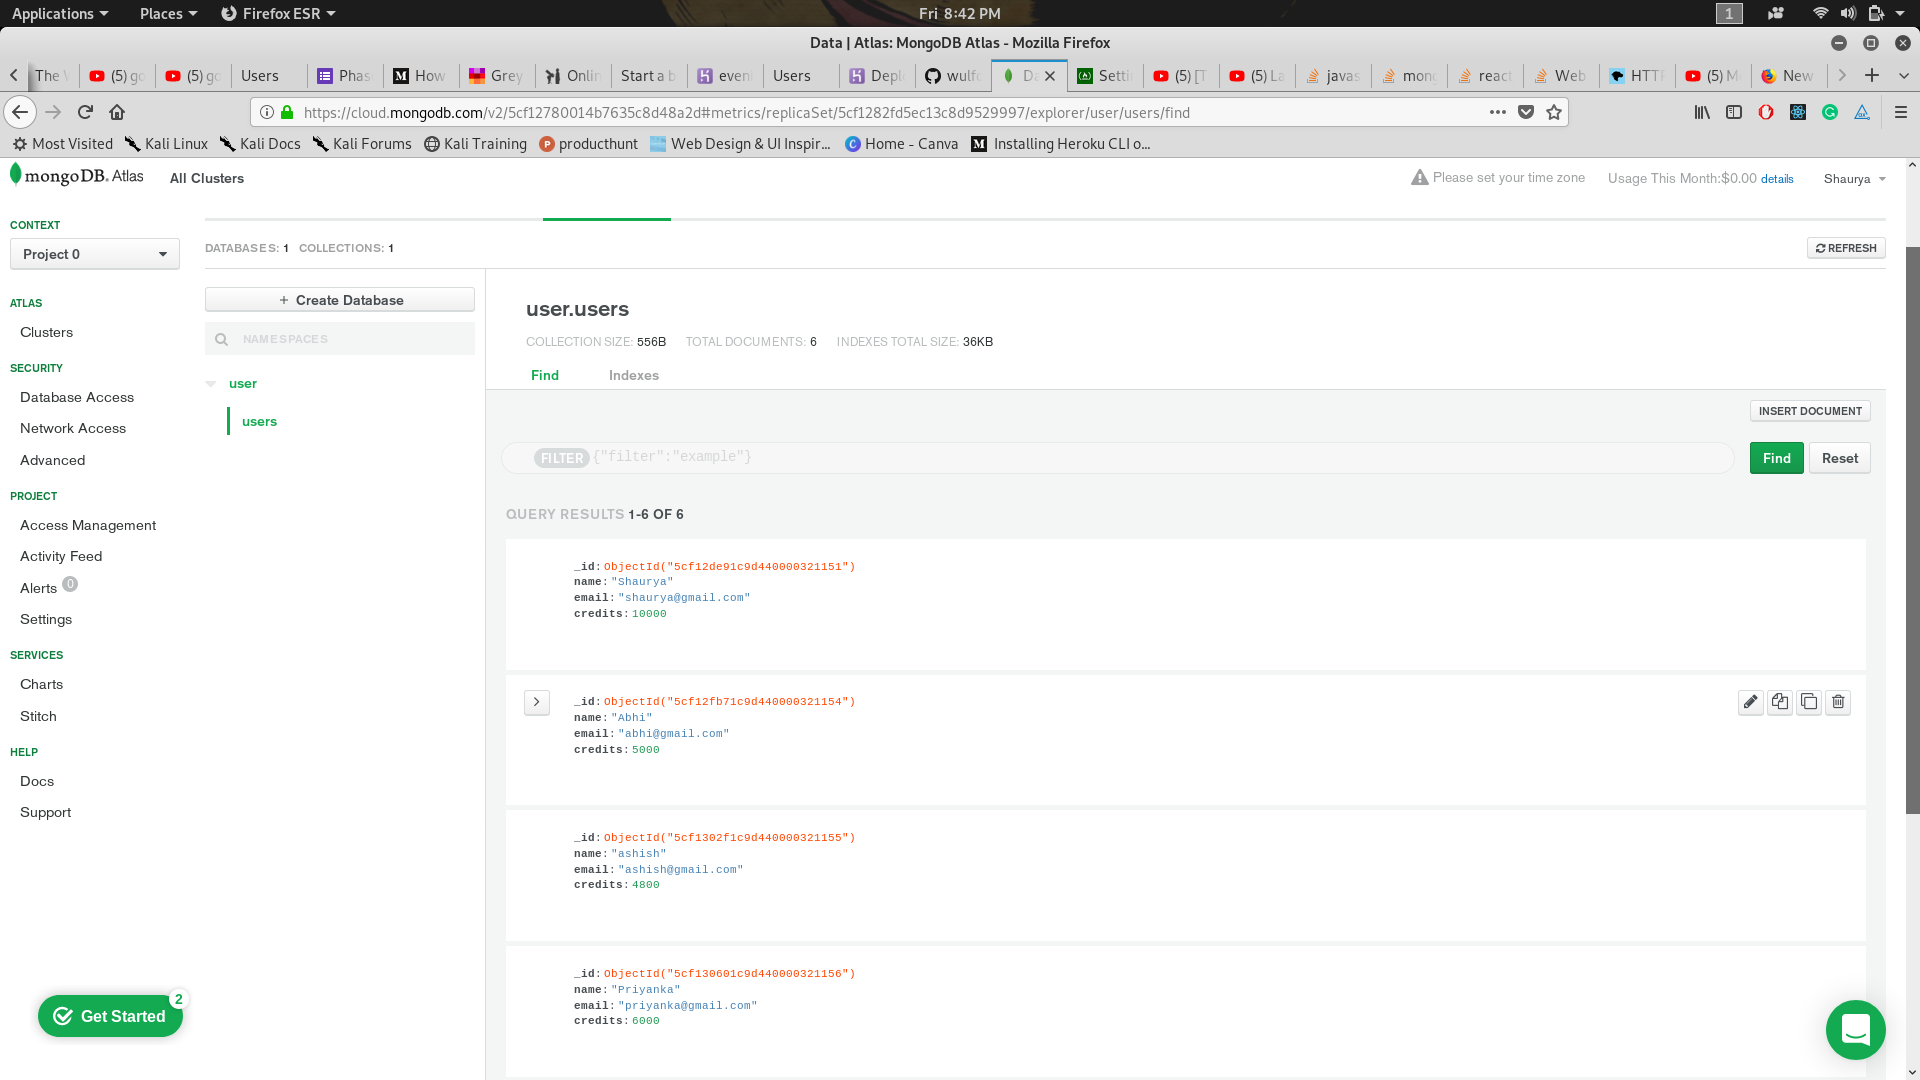
\includegraphics[width=0.85\textwidth]{images/related-work/monogo.png}
    \caption{Monogodb console}
    \label{fig:related_mongodb}
\end{figure}
\subsubsection{Firebase}
Firebase connects directly to client applications---web, iOS, or Android---through SDKs. When an app writes or reads data, Firebase automatically synchronizes changes in real time across all connected clients. The infrastructure handles scaling, replication, and offline support, so developers don’t need to manage servers. Security rules and authentication integrate directly with the database, making it simple to control access at a fine-grained level.

\begin{figure}[H]
    \centering
    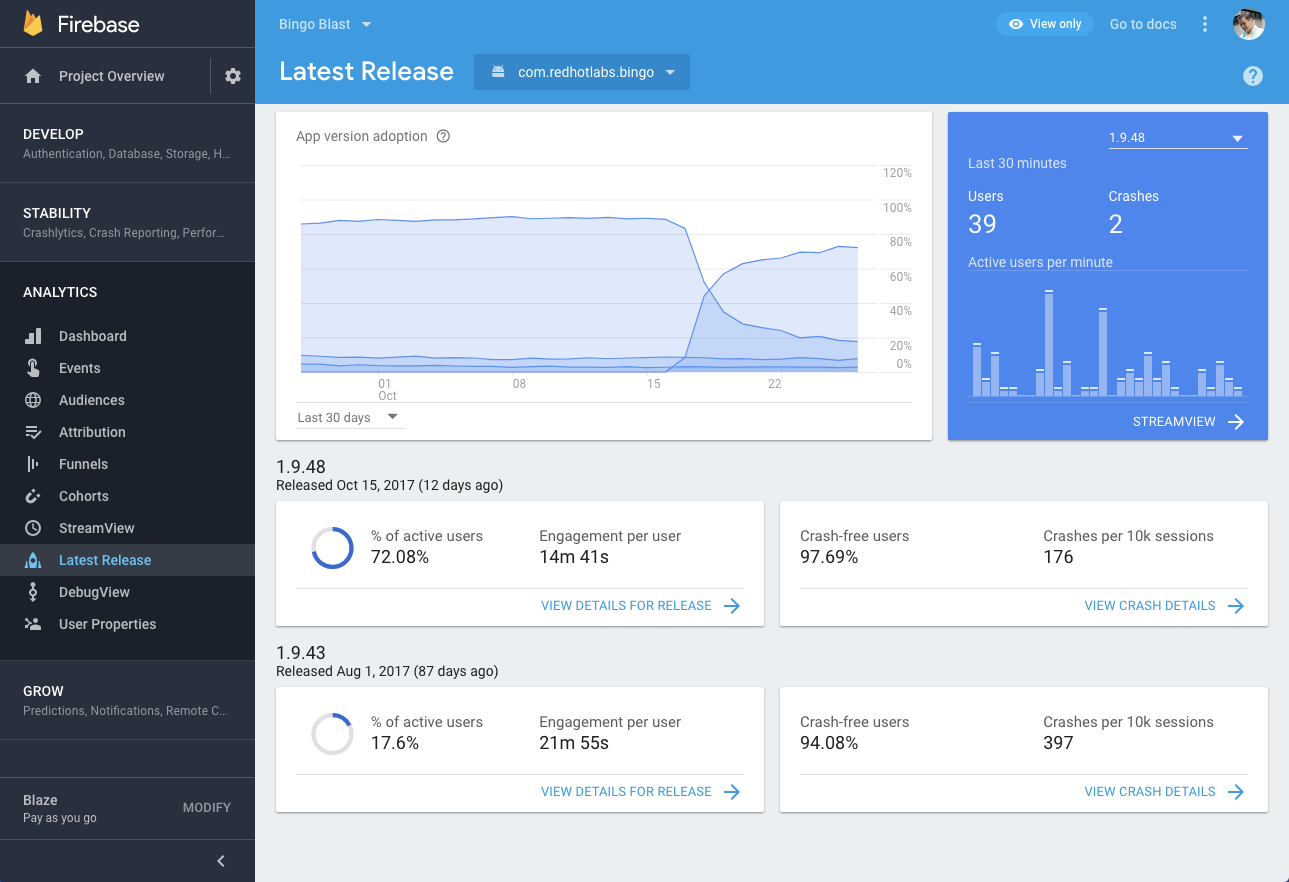
\includegraphics[width=0.85\textwidth]{images/related-work/firebase.png}
    \caption{Firebase console}
    \label{fig:related_firebase}
\end{figure}

\subsubsection{Supabase}
Supabase uses PostgreSQL as its core, but adds an API layer on top, exposing RESTful and GraphQL endpoints for applications. Applications can also subscribe to real-time changes via websockets. Supabase manages the database infrastructure, real-time updates, authentication, and storage. This means developers can interact both with SQL queries and API calls without managing servers. Real-time subscriptions allow applications to instantly react to database changes, similar to Firebase, while keeping the benefits of a structured relational database.

\begin{figure}[H]
    \centering
    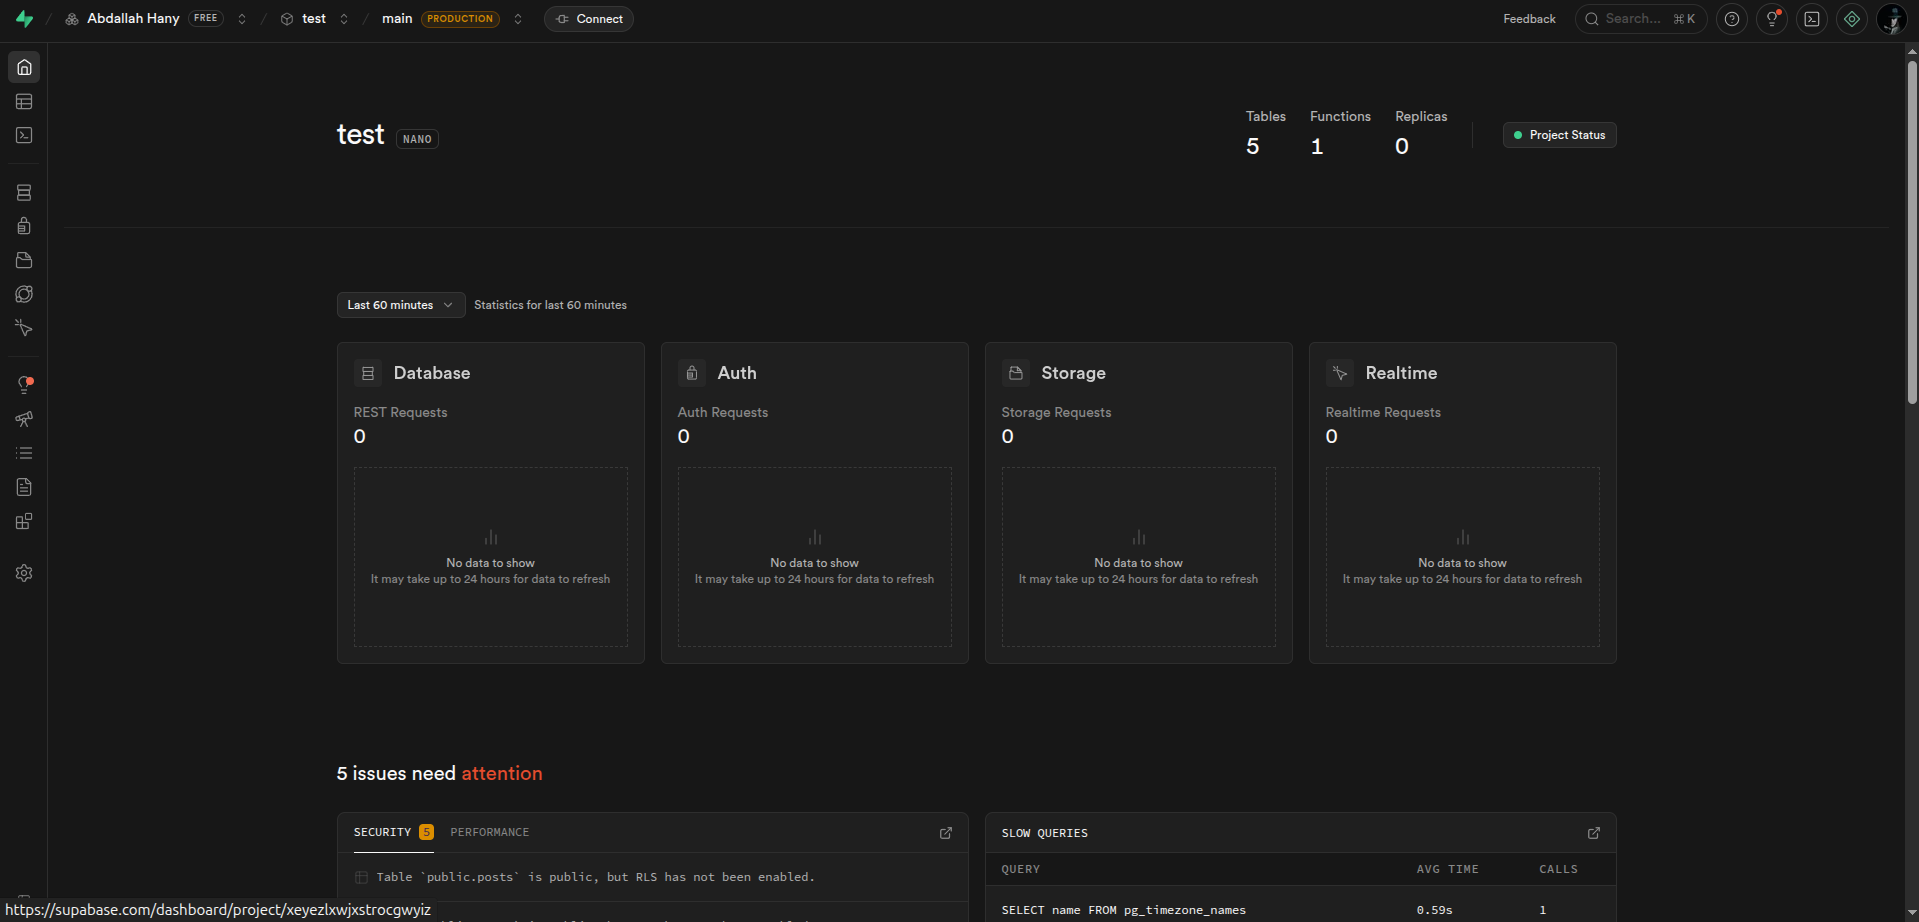
\includegraphics[width=0.85\textwidth]{images/related-work/supabase.png}
    \caption{Supabase console}
    \label{fig:related_supabase}
\end{figure}